% Use the following line _only_ if you're still using LaTeX 2.09.
%\documentstyle[icml2011,epsf,natbib]{article}
% If you rely on Latex2e packages, like most moden people use this:
\documentclass{article}

% For figures
\usepackage{graphicx} % more modern
%\usepackage{epsfig} % less modern
\usepackage{subfigure} 

% For citations
\usepackage{natbib}

% For algorithms
\usepackage{algorithm}
\usepackage{algorithmic}

% As of 2010, we use the hyperref package to produce hyperlinks in the
% resulting PDF.  If this breaks your system, please commend out the
% following usepackage line and replace \usepackage{icml2011} with
% \usepackage[nohyperref]{icml2011} above.
\usepackage{hyperref}

% Packages hyperref and algorithmic misbehave sometimes.  We can fix
% this with the following command.
\newcommand{\theHalgorithm}{\arabic{algorithm}}

% Employ the following version of the ``usepackage'' statement for
% submitting the draft version of the paper for review.  This will set
% the note in the first column to ``Under review.  Do not distribute.''
\usepackage[accepted]{icml2011} 
% Employ this version of the ``usepackage'' statement after the paper has
% been accepted, when creating the final version.  This will set the
% note in the first column to ``Appearing in''
% \usepackage[accepted]{icml2011}


% The \icmltitle you define below is probably too long as a header.
% Therefore, a short form for the running title is supplied here:
\icmltitlerunning{Context Aware Movie Recommender Systems}

\begin{document} 

\twocolumn[
\icmltitle{CAMR - Context Aware Movie Recommender Systems}

% It is OKAY to include author information, even for blind
% submissions: the style file will automatically remove it for you
% unless you've provided the [accepted] option to the icml2011
% package.
\icmlauthor{Primal Pappachan}{primal1@umbc.edu}
 %\icmladdress{Your Fantastic Institute,
%            314159 Pi St., Palo Alto, CA 94306 USA}
\icmlauthor{Arnav Joshi}{arnavj1@umbc.edu}
%\icmladdress{Their Fantastic Institute,
%            27182 Exp St., Toronto, ON M6H 2T1 CANADA}

% You may provide any keywords that you 
% find helpful for describing your paper; these are used to populate 
% the "keywords" metadata in the PDF but will not be shown in the document
\icmlkeywords{recommender systems, machine learning}

\vskip 0.3in
]

\section{Introduction}
The task of recommender systems is to turn data on users and their preferences into predictions of possible future likes and interests \cite{adomavicius2011context}.  The majority of existing approaches to recommender systems focuses on recommending the most relevant items to individual users. However, they do not take into consideration any contextual information, such as time, place and the company of other people (in use cases such as movies). In other words, traditional recommender systems deal with applications having only two types of entities, users and items, and do not put them into a context when providing recommendations. 
Context information is any information about the situation, circumstances and user state when a user is consuming the content item. Context can be the time of day, weather, social situation, user’s mood etc.\cite{segaran2008programming} However, the relationship between context and user decision making is very complex and difficult to model. 
Context-aware recommender systems help users and their desired content in a reasonable time, by exploiting the pieces of information that describe the situation in which users will consume the items. CAMRS models this approach by providing the recommendation on the basis of a function of user, item, previous ratings, as well as the context information provided of the user.

\subsection{Importance of context} 
The inclusion of the contextual information into the recommendation process presents opportunities for richer and more diverse interactions between the end-users and recommender systems. With the help of user's context, CAMRS will not only incorporate the user's profile of previous movies he has watched, but also include domain-dependent context modeling, which will help give better recommendation on the selection of movies.  Adapting the item choice based on the user's context can help give us better ratings for each movie recommendation.

\subsection{Collaborative Filtering}
Collaborative filtering systems gather item ratings as a form of user feedback for items in a given domain and exploit similarities and differences among profiles of several users in determining how to recommend an item. In movie recommendation, users provide ratings for the movies they have watched. 
A rating function in a recommendation system is one which tries to estimate the rating for the new item (here, the movie choice) based on the user's profile i.e. previous preferences.
This is done by initially generating a two-dimensional User x Item recommender matrix which takes partial user preference data as its input and produces a list of recommendations for each user as an output.
After the recommendation function is defined (or constructed) based on the available data, recommendation list for any given user u is typically generated by using the recommendation function on user u and all candidate items to obtain a predicted rating for each of the items and then by ranking all items according to their predicted rating value.
In CAMRS we hope to gain additional insight on user preferences by taking contextual information into consideration as explicit categories of data, such as the time, location and social situation(with a companion or not). The rating function r can thus be defined as: 
\begin{equation}r: User x Item x Context = Rating 
\end{equation}
The recommendation will be on a Likert scale (scale of 1-5) and detection of movie relevance is done on the basis of rating information. 

%\subsection{Content-based Filtering}
%Content based filtering methods provide recommendations by comparing representations of content contained %in an item to representations of content that interests the user.

\subsection{Post Filtering based on contextual attributes}
CAMRS generates recommendations based on contextual post-filtering. Post-filtering is a type of neighborhood-based algorithm, where a subset of users is chosen based on their similarity to the active user (the context is initially ignored). The resulting set of recommendations is adjusted (contextualized) for each user using the contextual information. The algorithm can be summarized in the following steps:
\begin{enumerate}
 \item Similarity between users is measured as the Pearson correlation between their ratings vectors.
 \item Select n users that have the highest similarity with the active user.
 \item Compute a prediction from a weighted combination of the selected neighbors ratings.
\end{enumerate}

\section{Related Work}
\cite{melville2002content} incorporated both content based and collaborative filtering methods for recommender systems. Their approach uses a content-based predictor to enhance existing user data, and then provide personalized suggestions through collaborative filtering. Collaborative filtering systems are affected by two problems:
\begin{description}
\item[Sparsity] Due to overwhelming amount of choices, the user-item rating matrix is sparse. Hence finding a sizable amount of similar ratings for the active user is usually low.\item[First-rater problem] An item can be recommended only when it is previously rated by a user.
\end{description}
The drawbacks for Collaborative Filtering (CF) systems were mitigated by exploiting content information of the items already rated. The basic approach uses content-based predictions to convert a sparse user ratings matrix into a full ratings matrix; and then uses CF to provide recommendations. The approach introduces a new model - Content-Boosted Collaborative Filtering (CBCF). The approach was proven to perform better than both pure content-based and collaborative filtering approaches.

\cite{adomavicius2011context} identifies the impact of context on recommender systems, models and predicts user tastes and preferences by incorporating available contextual information into the recommendation process as explicit additional categories of data. The approach also introduces three different algorithmic paradigms – contextual pre-
filtering, post-filtering, and modeling – for incorporating contextual information into the recommendation process. The contextual post-filtering paradigm is of significance, which uses a two-fold technique for filtering results:
\begin{description}
\item[Filtering] the recommendations such that only the items which are relevant to the active user are retained.
\item[Adjusting] the ranking of recommendations based on the context filters applied on the filtered results.
\end{description}
Further, they discuss the possibilities of combining several context- aware recommendation techniques into a single unifying approach.

\section{Proposed method}
The proposed method for building the CAMR system is to initially build a simple recommendation system that does not take the context under consideration. This model will take a part of the dataset for training, and predict the recommendation (ranked based on rating) for the given test instance using cross-validation. The next phase will include establishing a correlation between the contextual attributes and the rest of the features for finding a trend for a contextually richer movie recommendation. The final step will be to filter the instances based on the context attributes and provide a recommendation. Figure ~\ref{archdiag} shows the overall architecture of the recommendation system. The blocks \textit{U} represent the user input for the recommender matrix and \textit{C} represents the context for the post-filtering step. The correlation metric helps refine the context attribute for the filtering approach.  The following sections describe each of these steps.

\begin{figure}[H]
\centering
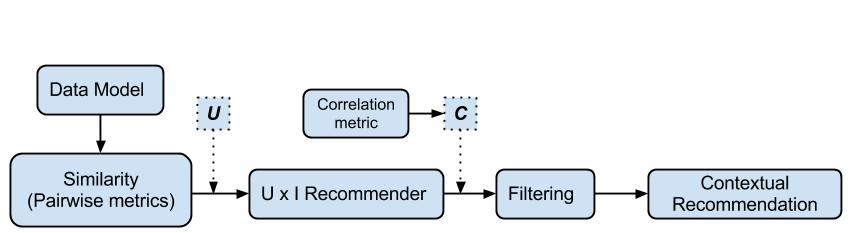
\includegraphics[width=3.5in]{archdiagram.jpg}
\caption{Contextual post-filtering for recommendation systems}
\label{archdiag}
\end{figure}

\subsection{Dataset}
We plan to use the LDOS - CoMoDa \cite{kovsir2011database} dataset, made available by Dr. Andrej Kosir from the University of Ljubljana, Slovenia. The LDOS - CoMoDa dataset is a context-rich movie recommender dataset, which contains ratings for movies along with contextual information describing the situations in which the movies were watched. 
It contains 30 variables among which are 12 contextual variables. The attributes can be classified as:
\begin{enumerate}
\item \emph{User Attributes}: ID, Sex, Age, City, Country
\item \emph{Movie Metadata}: rating, director, language, country, genre(s), actor(s), budget
\item \emph{Context attributes}: time,weather, daytype, season, location, social, end emotion, dominant emotion, mood, physical
\end{enumerate}
The value for each non-numerical discrete attribute is represented with a distinct number. The training instances for the recommendation system consists of the user, movie and context attributes for a single user and the corresponding rating associated with it. A single user can have multiple ratings, indicating he has rated more than one movie. The dataset consists of 2296 instances (ratings), with 121 unique users. 

\subsection{Simple recommendation system}
In the simple recommendation system, the contextual attributes for user profiles are ignored. Considering the user's attributes and the movie features (including the rating), the model calculates the similarity score between pairs of users. This score can be calculated by the Pearson correlation co-efficient. Based on this similarity score, the active user (the test instance) will be recommended movies from the users with a high similarity score with it. The recommendation will be based on a ranked list of movies. The ranking will be done as a function of the rating and the similarity score among the active user and the users having higher similarity scores. The accuracy will be determined based on the precision-recall calculation for the recommendations generated for the test user profile and the movies already rated by the user. 
%\subsubsection{Dictionaries}
The proposed method plans to maintain two separate dictionaries for user attributes (indexed by the user ID) and movie attributes (indexed by the movie ID). The movie attributes are mapped to individual users by the movie ID, as part of the values associated with each user instance.
%\subsubsection{Ranked list of recommendations}

\subsection{Correlation between context attributes}
The second step involves establishing a correlation among the contextual attributes and the attributes of a movie, as well as features related to the user. This helps determine the relevance of the contextual attribute for the movie recommendation to the user. This step helps in the process of selecting attributes which would be later used for post-filtering, thereby providing refined results. Based on experimentation, we establish a relationship among different contextual, user and movie attributes. The attributes that provide a better insight on the recommendation, based on their specific combinations and values, are more relevant in the post-filtering 

\subsection{Filtering of recommendations based on relevant context attributes}
In this stage, the model will generate a recommendation of movies for a particular test user instance. A single test instance would be a user profile, for which certain movie ratings that were present are removed. Using a precision-recall method, the predicted movie recommendations along with their corresponding ratings will be compared with this removed ratings for calculating the accuracy of predictions.

\section{Experiments}
\begin{table}
	\caption{LDOS - CoMoDa dataset statistic}
	\centering    
    \begin{tabular}{l|l}
    \hline
    \\
    Number of users            & 89 \\
    Number of items            & ~  \\
    Number of ratings          & ~  \\
    Average age                & ~  \\
    Number of countries        & ~  \\
    Number of cities           & ~  \\
    Max ratings of single user & ~  \\
    Min ratings of single user & ~  \\
    \end{tabular}
    \label{ldos}
\end{table}

\section{Conclusions}

\bibliography{pr_ref}
\bibliographystyle{icml2011}

\end{document} 
